\subsection{Neural dynamics}
\label{sec:neural-dynamics}

A common approach to systematically simulate a PING network involves the definition of neural dynamics through the Izhikevich type neuron model  \cite{Izhikevich2003}. This model is biologically plausible enough to mimic genuine neural behavior, yet it is computationally more efficient for large-scale simulations than more biophysically accurate models. There, every neuron is a dynamical system that can be described with a two-dimensional system of ordinary differential equations: for all $v \in V$,
\begin{align}
    \frac{dp_v}{dt} =\ & 0.04 p_v^2 + 5p_v + 140 - r_v + I_v,
    \label{eq:Izhikevich-model-dv-dt} \\
    \frac{dr_v}{dt} =\ & \alpha_{\type(v)} \cdot (\beta_{\type(v)} p_v - r_v), \label{eq:Izhikevich-model-dr-dt} \\
    \text{if } p_v \geq\ & p_{\thres} \text{, then } 
    \begin{cases}
        p_v \leftarrow \gamma_{\type(v)} \\
        r_v \leftarrow r_v + \zeta_{\type(v)}
    \end{cases}, 
    \label{eq:Izhikevich-model-p30}
\end{align}
where
\begin{itemize}
    \item $p_\thres$ is the threshold membrane potential ($= 30$ mV);
    
    \item $p$ represents the membrane potential of the neuron; 
    
    \item $r$ represents a membrane recovery variable, which dramatically increases after spikes; it provides negative feedback that suppresses the increase of $p$ and reduces the fluctuations in the output;
    
    \item $\alpha$ describes the timescale of $r$, it is proportional to the recovery speed;
    
    \item $\beta$ describes the sensitivity of $r$ to the subthreshold fluctuations of the membrane potential $p$: greater values of $\beta$ lead to stronger coupling between $p$ and $r$, resulting in more possible subthreshold oscillations;
    
    \item $\gamma$ describes the after-spike reset value of $p$;
    
    \item $\zeta$ describes the after-spike reset value of $r$;
    
    \item $I$ describes the current.
\end{itemize}
The constants in Equation (\ref{eq:Izhikevich-model-dv-dt}) have been obtained by fitting the spike initiation of neural dynamics in such a way that $p$ has a scale of \textit{mV}, and $t$ - a scale of \textit{ms}.
The effects the parameters $\alpha, \beta, \gamma, \zeta$ have on membrane potential and recovery are visualized in Figure \ref{fig:neural-dynamics}.

\begin{figure}
    \centering
    % ----- INPUT
\newcommand{\ndimagew}{0.4\textwidth}
\newcommand{\ndimageh}{0.75 * \ndimagew}


\begin{tikzpicture}[
        arr/.style = { -{Stealth[ ]} },
        bluearrow/.style = {arr, draw=third-color, fill=third-color, thick},
        blackarrow/.style = {arr, ultra thick},
    ]
    
    \begin{scope}
    % p(t), r(t)
    \node[] (pt) at (-0.5, 0) {$p(t)$};
    \node[] (rt) at (-0.5, 0.42 * \ndimageh) {$r(t)$};
    
    % peak
    \node[anchor=west] (peaktxt) at (1.1 * \ndimagew, \ndimageh) {\bgcolorsmalltext{third-color}{black}{peak ($30$ mV)}};
    \node[] (peak) at (0.4 * \ndimagew, \ndimageh) {};
    \path [bluearrow] (peaktxt) edge node {} (peak);
    
    % decay alpha 
    \node[anchor=west] (decaytxt) at (1.1 * \ndimagew, 0.2 * \ndimageh) {\bgcolorsmalltext{third-color}{black}{decay with rate $\alpha$}};
    \node[] (decay) at (0.6 * \ndimagew, 0.2 * \ndimageh) {};
    \path [bluearrow] (decaytxt) edge node {} (decay);
    
    % sensitivity beta
    \node[] (senstxt) at (0.6 * \ndimagew, -0.2 * \ndimageh) {\bgcolorsmalltext{third-color}{black}{sensitivity $\beta$}};
    \node[] (sens) at (0.35 * \ndimagew, 0.07 * \ndimageh) {};
    \path [bluearrow] (senstxt) edge node {} (sens);
    
    % reset gamma
    \node[anchor=west] (resetgtxt) at (1.1 * \ndimagew, 0.52 * \ndimageh) {\bgcolorsmalltext{third-color}{black}{reset $\gamma$}};
    \node[] (resetg) at (0.42 * \ndimagew, 0.52 * \ndimageh) {};
    \path [bluearrow] (resetgtxt) edge node {} (resetg);
    
    % reset zeta
    \node[] (resetztxt) at (0.1 * \ndimagew, 0.2 * \ndimageh) {\bgcolorsmalltext{third-color}{black}{reset $\zeta$}};
    \node[] (resetz) at (0.39 * \ndimagew, 0.2 * \ndimageh) {};
    \path [bluearrow] (resetztxt) edge node {} (resetz);
        
    \end{scope}
    
    \begin{scope}
        \node[anchor=south west,inner sep=0] at (0,0) {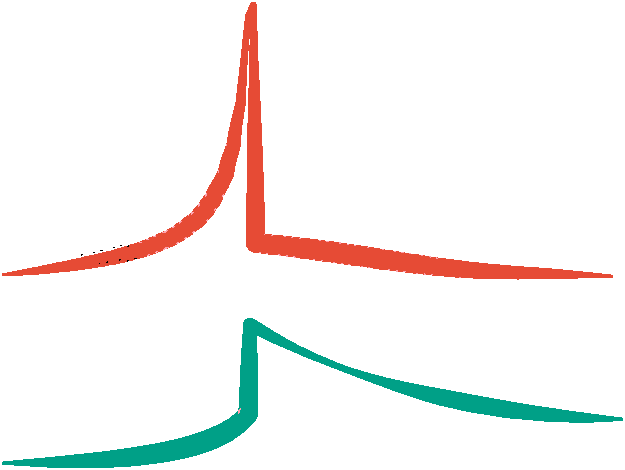
\includegraphics[width=\ndimagew]{src/assets/images/neural-dynamics.png}};
    \end{scope}
        
\end{tikzpicture}
    \caption{Effects of parameters on neural dynamics in the Izhikevich model. {\it This figure is reproduced with permission from \url{www.izhikevich.com}. (Electronic version of the figure and reproduction permissions are freely available at \url{www.izhikevich.com.})}}
    \label{fig:neural-dynamics}
\end{figure}

The parameters $\alpha, \beta, \gamma, \zeta$ correspond to known types of neurons. The parameters' values for regular spiking (RS) excitatory and fast spiking (FS) inhibitory neurons used in this thesis are displayed in Table \ref{tab:params-izhikevich-model}. When a stimulus is applied, RS neurons typically first fire with a short interspike period, which later increases (see Figure \ref{fig:neuron-types-rs}). Thus, this neuron type corresponds to the large value of $\zeta$, which causes an after-spike jump in $r$. FS neurons produce periodic spikes with high frequency, hence the extremely low value of $\alpha$, which allows for fast recovery (see Figure \ref{fig:neuron-types-fs}).

\begin{table}[!htp] 
    \centering
    \begin{tabular}{|
    >{\columncolor{table-color}}c |c|c|}
    \hline
    \textbf{Parameter}      & \cellcolor{table-color}\textbf{$\pmb{\ex}$ - Regular spiking (RS)} & \cellcolor{table-color}\textbf{$\pmb{\inh}$ - Fast spiking (FS)} \\ \hline
    \textbf{$\pmb{\alpha}$} & 0.02                                                               & 0.1                                                             \\ \hline
    \textbf{$\pmb{\beta}$}  & 0.2                                                                & 0.2                                                             \\ \hline
    \textbf{$\pmb{\gamma}$} & -65                                                                & -65                                                             \\ \hline
    \textbf{$\pmb{\zeta}$}  & 8                                                                  & 2                                                               \\ \hline
\end{tabular}
    \caption{Parameters of the Izhikevich model for regular and fast spiking neurons \cite{Izhikevich2003}.}
\label{tab:params-izhikevich-model}
\end{table}

\begin{figure}[!htp]
\hspace*{-1.5cm} 
    \centering
    \begin{subfigure}[t]{0.3\textwidth}
        \centering
        % ----- INPUT
\newcommand{\rsimagew}{\textwidth}
\newcommand{\rsimageh}{0.833 * \rsimagew}


\begin{tikzpicture}
    
    \begin{scope}
        \node[] (It) at (-0.5, 0) {$I(t)$};
        \node[] (pt) at (-0.5, 0.22 * \rsimageh) {$p(t)$};
    \end{scope}
    
    \begin{scope}
        \node[anchor=south west,inner sep=0] at (0,0) {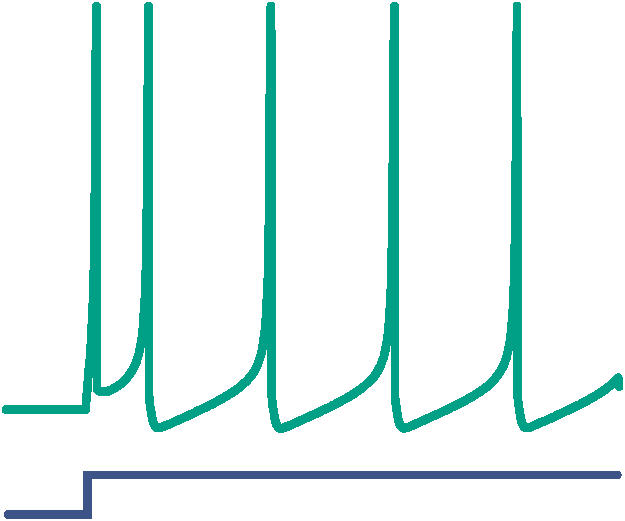
\includegraphics[width=\rsimagew]{src/assets/images/neuron-types/neuron-types_RS.png}};
    \end{scope}
        
\end{tikzpicture}
        \caption{{Regular spiking (RS).}}
        \label{fig:neuron-types-rs}
    \end{subfigure}
    \hspace{0.1\textwidth}
    \begin{subfigure}[t]{0.3\textwidth}
        \centering
        % ----- INPUT
\newcommand{\fsimagew}{\textwidth}
\newcommand{\fsimageh}{0.833 * \fsimagew}

\begin{tikzpicture}
    
    \begin{scope}
        \node[] (It) at (-0.5, 0) {$I(t)$};
        \node[] (pt) at (-0.5, 0.22 * \fsimageh) {$p(t)$};
    \end{scope}
    
    \begin{scope}
        \node[anchor=south west,inner sep=0] at (0,0) {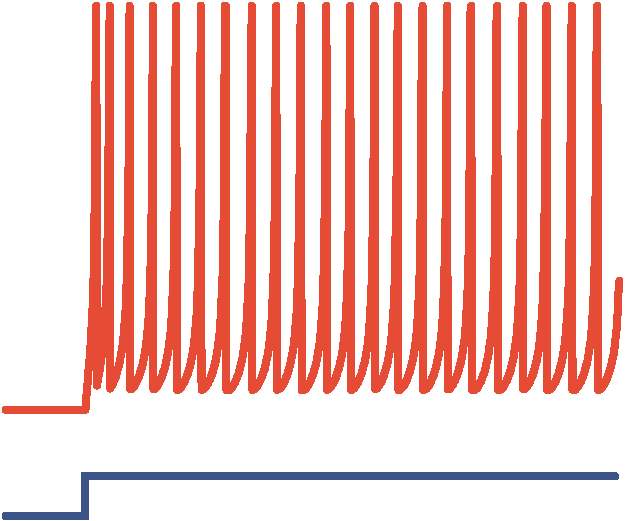
\includegraphics[width=\fsimagew]{src/assets/images/neuron-types/neuron-types_FS.pdf}};
    \end{scope}
        
\end{tikzpicture}
        \caption{Fast spiking (FS).}
        \label{fig:neuron-types-fs}
    \end{subfigure}
    \caption{Spiking behavior of neurons regular and fast spiking neurons in the Izhikevich model. Each horizontal bar represents 20 ms of simulation. {\it This figure is reproduced with permission from \url{www.izhikevich.com}. (Electronic version of the figure and reproduction permissions are freely available at \url{www.izhikevich.com.})}}
    \label{fig:neuron-types}
\end{figure}

\paragraph{Current composition}

In the network, neurons are not isolated, and the current ($I_v$) in Equation (\ref{eq:Izhikevich-model-dv-dt}) involves the accumulated effect of interactions with other neurons. Hence, the equation must include the input current ($I_{\stim}$) as well as the coupling weights between the neurons ($K$), and the effects of synaptic potentials GABA-A (inhibitory) and AMPA (excitatory; $I_{\syn}$):
\begin{gather}
    I_v = 
    \sum_{w \in V} \cost_{(v \to w)} + I_{\stim, v} \mathbb{1} \{ \type(v) = \ex \},  \label{eq:current-components} \\
    \cost_{(v \to w)} = K_{v, w} \cdot I_{\syn, w}. 
    \label{eq:cost-function}
\end{gather}

In this project, the external input ($I_{\stim}$) is provided by a set of texture stimuli, and a grid network of PING oscillators is supposed to reflect local neural networks of the primary visual cortex (V1). The external stimuli is described in Section \ref{sec:external-stimuli}.

\subsubsection{Coupling weights}
\label{sec:coupling-weights}

The interaction strength of lateral connections is represented by a matrix of coupling weights ($K$), in which $K_{v, w}$ is the coupling weight between the neurons $v$ and $w$. 
The coupling weight between each pair of neurons is defined by an exponential function decaying by the euclidean distance between the oscillators they belong to. The PING networks in Figure \ref{fig:oscillatory-grid-graph} are reduced to the point oscillators as portrayed in Figure \ref{fig:oscillatory-point-grid}. 
Let $\loc: V \to \mathbb{N}^2$ be a function mapping a neuron to the position of the oscillator it belongs to in the grid. Then the coupling weigh between the neurons $v$ and $w$ is
\begin{equation}
    K_{v, w} = C_{\type(v) \to \type(w)} \exp \left( \frac{-\| \loc(v), \loc(w) \|}{s_{\type(v) \to \type(w)}} \right),
    \label{eq:coupling-weights}
\end{equation}
where $C$ and $s$ are connectivity dependent values representing the maximum connection strength between neurons and the decay rate of connectivity over space, respectively. The values for these constants are presented in Table \ref{tab:connectivity-network-constants}.

\begin{figure}[!htp]
    \centering
    \begin{tikzpicture}[
    cnode/.style = {circle,thick,fill=color-two}
]
    
    
    \begin{scope}[>={Stealth[black]}]
        % vertical 
        
        \draw (0, 0) to (0, 1);
        \draw (0, 1) to (0, 2);
        \draw (1, 0) to (1, 1);
        \draw (1, 1) to (1, 2);
        \draw (2, 0) to (2, 1);
        \draw (2, 1) to (2, 2);
        
        % horizontal 
        
        \draw (0, 0) to (1, 0);
        \draw (1, 0) to (2, 0);
        \draw (0, 1) to (1, 1);
        \draw (1, 1) to (2, 1);
        \draw (0, 2) to (1, 2);
        \draw (1, 2) to (2, 2);
    \end{scope}
    
    \begin{scope}
        
        \node[style=cnode] (V1) at (0, 0) {};
        \node[style=cnode] (V2) at (0, 1) {};
        \node[style=cnode] (V3) at (0, 2) {};
        \node[style=cnode] (V4) at (1, 0) {};
        \node[style=cnode] (V5) at (1, 1) {};
        \node[style=cnode] (V6) at (1, 2) {};
        \node[style=cnode] (V7) at (2, 0) {};
        \node[style=cnode] (V8) at (2, 1) {};
        \node[style=cnode] (V9) at (2, 2) {};
    \end{scope}


\end{tikzpicture}
    \caption{A 3 $\times$ 3 oscillatory network, where each PING network is a point.}
    \label{fig:oscillatory-point-grid}
\end{figure}

\begin{table}[!htp] 
    \centering
    \begin{tabular}{|
    >{\columncolor{main-color}}c|c|c|}
    \hline
    \textbf{Connectivity} & \cellcolor{main-color}\textbf{Spatial constant $\pmb{s}$} & \cellcolor{main-color}\textbf{Max connection strength $\pmb{C}$} \\ \hline
    \textbf{$\pmb{\ex \to \ex}$}    & 0.4                                                         & 0.004                                                              \\ \hline
    \textbf{$\pmb{\ex \to \inh}$}    & 0.3                                                         & 0.07                                                               \\ \hline
    \textbf{$\pmb{\inh \to \ex}$}    & 0.3                                                         & -0.04                                                              \\ \hline
    \textbf{$\pmb{\inh \to \inh}$}    & 0.3                                                         & -0.015                                                             \\ \hline
\end{tabular}
    \caption{The constants of the network connectivity \cite{Lowet2015}.}
    \label{tab:connectivity-network-constants}
\end{table}
\subsubsection{Synaptic potentials}
\label{sec:synaptic-potentials}

Let $v, w \in V$ be the pre- and postsynaptic neurons, respectively, and let $(v \to w) \in E$ be the electrically conductive link (synapse) between them. When a spike arrives at the synapse, it triggers the release of a neurotransmitter: AMPA when $\type(v) = \ex$, GABA when $\type(v) = \inh$ \cite{Lowet2015}. After firing an action potential, the voltage of the presynaptic neuron resets to its equilibrium potential, at which there is no net flow through its ionic channels \cite{JohnsBook2014:6}. The equilibrium potential is equal to the reversal (Nernst) potential (whereat the net current flow reverses its direction), which only depends on the type of the postsynaptic neuron, $P_\ex$ if $\type(w) = \ex$, $P_\inh$ if $\type(w) = \inh$. 

From Ohm's law, it follows that the current through a neuron is proportional to its conductance and driving force \cite{KandelBook2003:6}. The latter is the difference between the synapse's reversal (presynaptic neuron's equilibrium) and the neuron's membrane potentials. The conductance of a neuron is the sum of all synapses' conductances of that neuron. Additionally, each neuron receives two synaptic inputs: from excitatory and inhibitory neurons. Therefore, the synaptic current of a postsynaptic neuron $w$ is
\begin{equation}
    I_{\syn, w} = G_{\inh, w} (p_{w} - P_{\inh}) + G_{\ex, w} (p_{w} - P_{\ex}),
    \label{eq:synaptic-current}
\end{equation}
where $P_w$ is the neural membrane potential, and $G_{\inh}$ and $G_{\ex}$ are total synaptic conductances from the inhibitory and excitatory presynaptic neurons, respectively \cite{Lowet2015}, \cite{Jensen2005}. The former is of the form 
\begin{equation}
    G_{\inh, w} = \sum_{v \in V: \type(v) = \inh} g_{\inh \to \type(w)} \cdot s_{(v \to w)},
    \label{eq:total-synaptic-conductance-in},
\end{equation}
where $g$ is the conductance density of the GABA-mediated receptor between a pair of neurons, the values of which are displayed in Table \ref{tab:conductance-synaptic}, and $s$ is the synaptic gating value. The expression for the excitatory synaptic conductance $G_{\ex, v}$ is analogous to Equation (\ref{eq:total-synaptic-conductance-in}).

A synaptic gate can be though of as a transistor that modifies the conductance of a synapse, it can amplify and switch electrical signals. The gating value includes the rise $\rho$ and decay $\tau$ times and the transmission concentration term to mediate the interneural signal transmission \cite{Destexhe1994}:
\begin{equation}
    \frac{ds_{(v \to w)}}{dt} = \rho_{(v \to w)} \underbrace{\left( 1 + \tanh \left( \frac{p_{w}}{4} \right) \right)}_{T_w: \text{trans. conc.}} (1 - s_{(v \to w)}) - \frac{s_{(v \to w)}}{\tau_{(v \to w)}}.
    \label{eq:synaptic-gates2}
\end{equation}
For a given neuron, it is assumed that the dynamics of all its synapses are synchronized. Therefore, although a synaptic gate is located on the postsynaptic neuron $w$, it follows the potential and gating parameters of the presynaptic neuron $v$ \cite{Lowet2015}. Hence, Equation (\ref{eq:synaptic-gates2}) is equivalent to
\begin{equation}
    \frac{ds_{(v \to w)}}{dt} = \rho_{v} \underbrace{\left( 1 + \tanh \left( \frac{p_{v}}{4} \right) \right)}_{T_v: \text{trans. conc.}} (1 - s_{(v \to w)}) - \frac{s_{(v \to w)}}{\tau_{v}}.
    \label{eq:synaptic-gates}
\end{equation}
The values for the synaptic parameters are presented in Table \ref{tab:synaptic-current-params}.
The initial value of the gating value is zero. The equation is separable, and, thus, its solution is
\begin{equation}
    s_{(v \to w)} = \frac{\rho_v T_v / \tau_v}{\rho_v T_v / \tau_v + 1} \exp \left( -t \cdot \tau_v (\rho_v T_v + 1)  \right).
\end{equation}
Since all the terms are positive, this solution is bounded below by $0$ and above by $1$.

As mentioned in Section \ref{sec:action-potential}, the spike initiating threshold for excitatory neurons is between $-60$ and $-40$ mV. When the neuron is at rest, that is $p_v < -40$ mV, the transmission concentration is at its minimum:
\begin{gather}
\begin{split}
    & T_v = 1 + \tanh \left( \frac{p_{v}}{4} \right) \approx 0 \\
    \Rightarrow \ & \frac{ds_{(v \to w)}}{dt} \approx - \frac{s_{(v \to w)}}{\tau_{v}}.
\end{split}
\end{gather}
This implies that the gating decays exponentially.
So, in between spikes, the conductance and thus the synaptic input from the neuron $v$ decreases. 

During an action potential, the membrane potential reaches $p_v > 10$. Thus, the transmission concentration is at its maximum, and
\begin{gather}
\begin{split}
    & T_v = 1 + \tanh \left( \frac{p_{v}}{4} \right) \approx 2 \\
    \Rightarrow \ & \frac{ds_{(v \to w)}}{dt} \approx 2 \cdot \rho_v (1 - s_{(v \to w)}) - \frac{s_{(v \to w)}}{\tau_{v}},
\end{split}
\end{gather}
which indicates that the gating rises during the action potential and falls once it is over. 

\begin{table}[!htp] 
    \centering
    \begin{tabular}{|
    >{\columncolor{main-color}}c|c|c|}
    \hline
    \textbf{Connectivity}                           & \cellcolor{main-color}\textbf{Conductance $\pmb{g}$} \\ \hline
    \textbf{$\pmb{\ex \to \ex}$}& 0.6                                                    \\ \hline
    \textbf{$\pmb{\ex \to \inh}$} & 0.06                                                   \\ \hline
    \textbf{$\pmb{\inh \to \ex}$} & 0.8                                                    \\ \hline
    \textbf{$\pmb{\inh \to \inh}$} & 0.5                                                    \\ \hline
\end{tabular}
    \caption{Synaptic conductance values \cite{Lowet2015}.}
    \label{tab:conductance-synaptic}
\end{table}

\begin{table}[!htp] 
    \centering
    \begin{tabular}{l|c|c|c|}
    \cline{2-4}
    \textbf{}                                                     & \cellcolor{table-color}\textbf{Reversal potential (mV)} & \cellcolor{table-color}\textbf{$\pmb{\rho_{j} \; \text{ (} ms^{-1} \text{)}}$} & \cellcolor{table-color}\textbf{$\pmb{\tau_{j} \text{ (} ms \text{)}}$} \\ \hline
    \multicolumn{1}{|l|}{\cellcolor{table-color}\textbf{AMPA}}   & $p_{\inh} = 0$                                             & $1$                                                                              & $2.4$                                                                       \\ \hline
    \multicolumn{1}{|l|}{\cellcolor{table-color}\textbf{GABA}} & $p_{\ex} = -80$                                           & $2$                                                                              & $20$                                                                        \\ \hline
\end{tabular}
    \caption{Synaptic parameter values for AMPA and GABA-A \cite{Lowet2015}.}
    \label{tab:synaptic-current-params}
\end{table}


